\chapter{The Cassini-Huygens Mission}
\label{chap:cassini}
\section{Overview}
%http://sci.esa.int/cassini-huygens/33415-summary/
The \textit{Cassini-Huygens} mission (hereafter known as \textit{Cassini}) was a space mission designed to investigate the Saturn system, and was a collaboration between NASA, ESA and the Italian Space Agency (ASI). It was composed of a main \textit{Cassini} orbiter spacecraft with 12 instruments on board, and the \textit{Huygens} probe with a further 6, as described in \citet{matson2002}. A diagram of this spacecraft is shown in Figure~\ref{cassini:fig:spacecraft}. The instruments particularly relevant to the work in this thesis are discussed later in this chapter. 

\begin{figure}
\centering
\noindent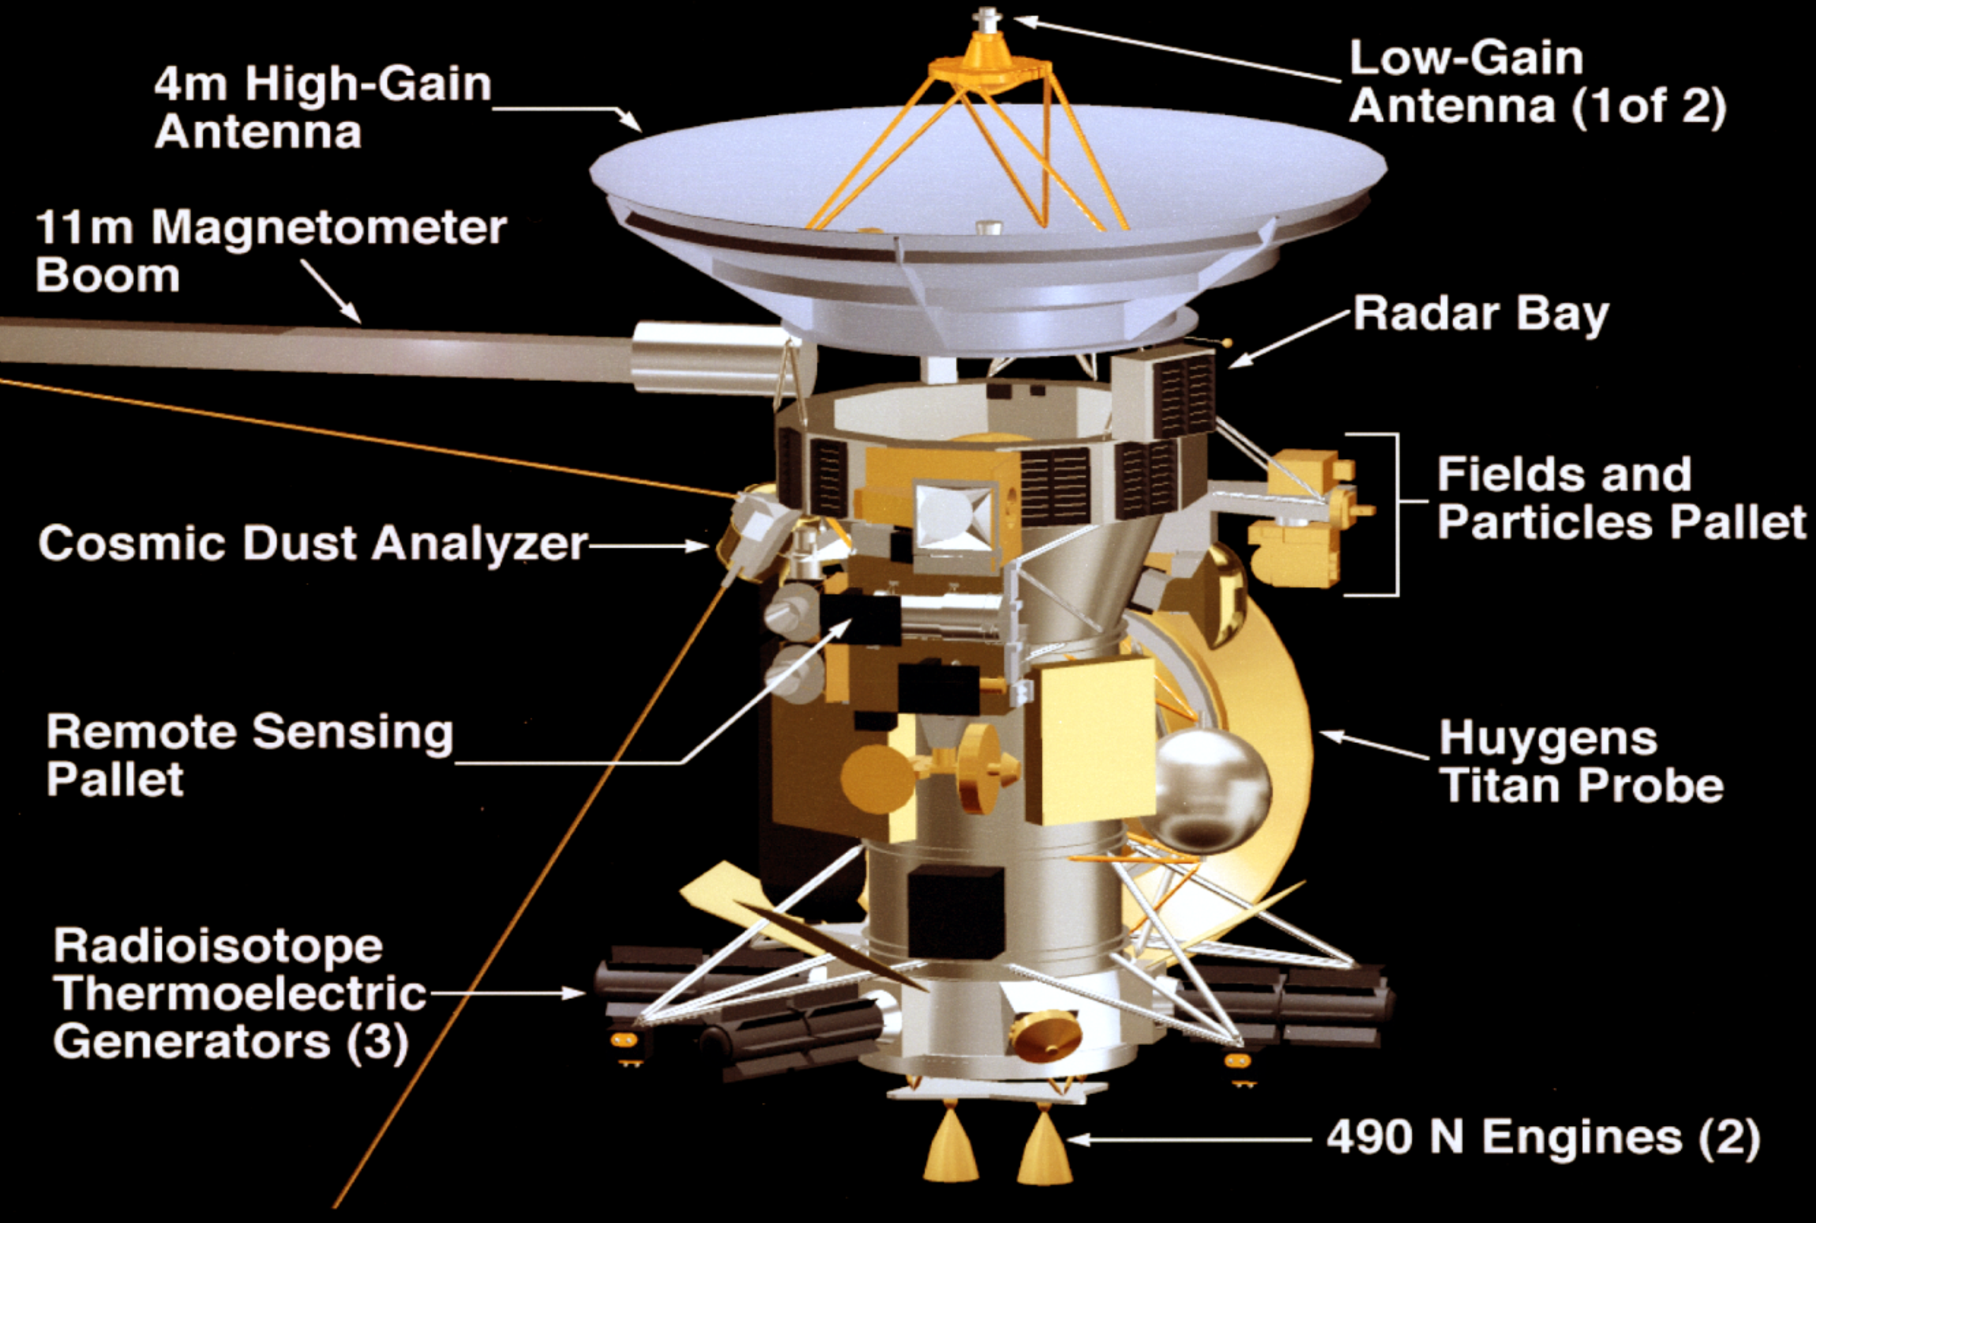
\includegraphics[width=0.9\textwidth]{cassini/spacecraft.pdf}
\caption[Diagram of the \textit{Cassini-Huygens} spacecraft]{Diagram of the \textit{Cassini-Huygens} spacecraft, from \citet{narvaez2004}. The spacecraft is about \SI{6.8}{m} in height.}
\label{cassini:fig:spacecraft}
\end{figure}

Together, these instruments were designed such that the mission could investigate the entire Saturn system, from the planet itself to its atmosphere, rings, moons, and magnetosphere. The moon Titan was one of the key focuses of the investigation, as it is the only moon in the solar system with a significant atmosphere, and it was initially thought to be a key source of plasma for the magnetosphere. The \textit{Huygens} probe was therefore designed to detach from the main \textit{Cassini} orbiter and make a single trajectory by parachute down to the surface of Titan, making \textit{in situ} measurements of Titan's atmosphere during the descent. The shield covering the \textit{Huygens} probe before it was deployed can be seen in Figure~\ref{cassini:fig:spacecraft}.

\section{Mission Timeline}
\textit{Cassini} launched from Cape Canaveral in Florida in October 1997, and finally arrived at the Saturn system in July 2004, after gravity-assist flybys of Venus, Earth and Jupiter. The mission was initially designed to operate for four years, from 2004-2008, and during this `Prime Mission' \textit{Cassini} completed 75 orbits of Saturn, and 44 flybys of Titan. The Prime Mission was incredibly successful, resulting in many exciting and unexpected discoveries about the Saturn system, such as the plumes of water being ejected from the icy moon Enceladus \citep{dougherty2006}. 

The mission was then extended by two years; the `Equinox Mission'. This extension allowed \textit{Cassini} to observe how the behaviour of the Saturn system changed with season, from northern winter to northern spring. Saturn's obliquity relative to the ecliptic plane is \SI{26.7}{\degree}. As discussed in Section~\ref{intro:sec:saturn}, a Saturn year lasts 29 years, and the northern spring equinox occurred in August 2009, near the middle of the Equinox Mission. From a magnetospheric science perspective, equinox is a particularly interesting time to investigate the Saturn system, as the incident solar wind direction is parallel to Saturn's rotational/dipole equator, rather than at an angle slightly above or below. This means the solar wind conditions are approximately symmetrical in the northern and southern hemispheres, allowing for certain hemispheric effects, such as those discussed in Section~\ref{intro:sec:periodicities}, to be more readily investigated. Indeed, the data that is analysed in this thesis, particularly in Chapter~\ref{chap:equinox}, were measured during \textit{Cassini's} Equinox Mission.

The mission was then further extended from 2010-2017, known as the `Solstice Mission', as the Saturn year continued into northern summer solstice in May 2017. The spacecraft trajectories were optimised to provide the most extensive coverage of scientifically interesting areas of the Saturn system, in the context of the entire mission. This culminated in the Grand Finale's `Proximal Orbits', from April to September 2017. In each of these 22 final orbits, \textit{Cassini} traversed the gap between Saturn's atmosphere and the innermost ring, therefore orbiting far closer to the planet than at any other time in the mission. This provided the opportunity to investigate scientific mysteries that still had not been answered from mission data so far, such as the core rotation rate of the planet and internal magnetic field structure. The \textit{Cassini} mission then ended on 15 September 2017, as the spacecraft plunged into the planet's atmosphere and lost contact with Earth. The Grand Finale was designed in this way not just for maximum scientific reward, but also because the onboard rocket propellant used to manoeuvre the spacecraft was running out. With \textit{Cassini's} discovery of a likely sub-surface water ocean at Enceladus, and also prebiotic chemistry at Titan, the mission could not risk the spacecraft accidentally crashing into one of these moons and potentially contaminating them with Earth-based life forms. It was therefore necessary to deliberately crash the spacecraft into the planet Saturn itself.

Figure~\ref{cassini:fig:missionoverview} shows an overview of the entire \textit{Cassini} mission. At the top of the image the trajectories of the orbits are depicted, showing the extensive coverage \textit{Cassini} made in radial distance, latitude and local time. Also shown are the number of flybys of various moons, and  at the bottom the Saturn season is depicted. The proximal orbits, shown in red, are barely visible as they are so close to the Saturn surface.

\begin{figure}
\centering
\noindent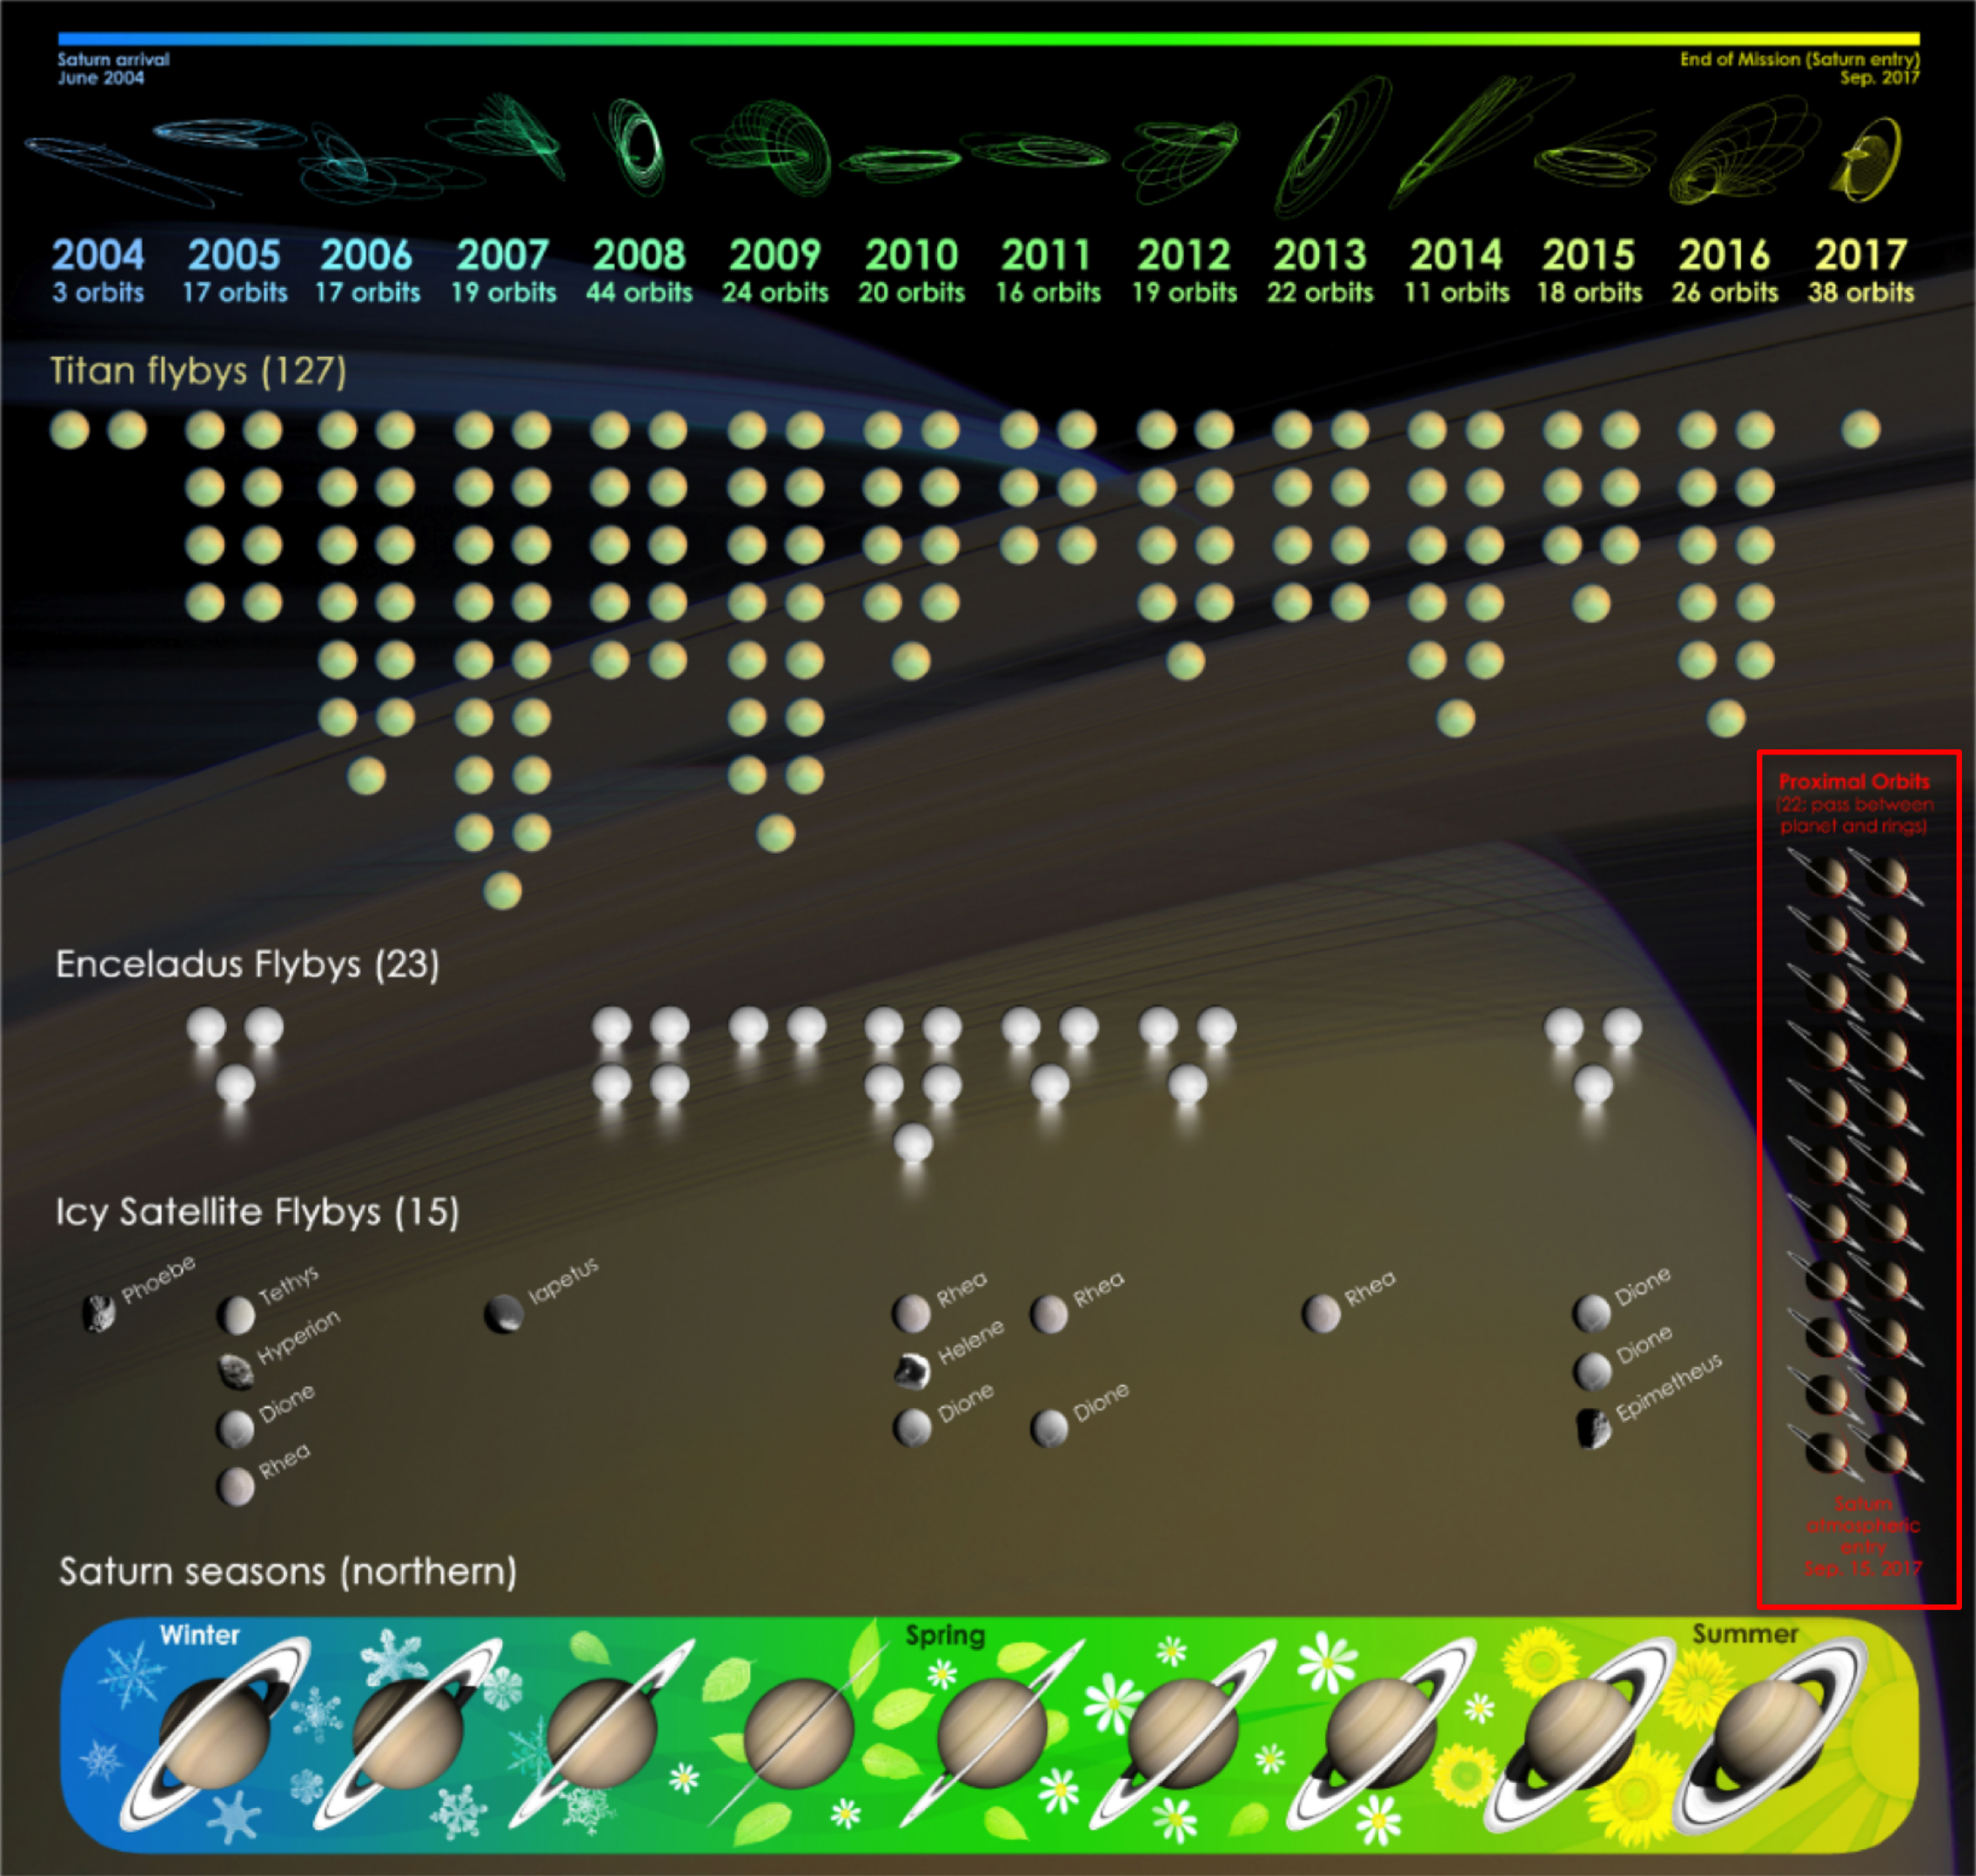
\includegraphics[width=0.9\textwidth]{cassini/mission_overview.jpg}
\caption[Diagram showing overview of \textit{Cassini }space mission.]{Diagram showing overview of \textit{Cassini} space mission orbit trajectories and moon flybys, from \citet{nasa2017}.}
\label{cassini:fig:missionoverview}
\end{figure}

\section{Key Instruments}
\subsection{Magnetometer (MAG)}
The dual technique magnetometer system (MAG) measured the magnitude and direction of Saturn's magnetic field \textit{in situ}, described in \citet{dougherty2004} and summarised here. The system was composed of a Vector/Scalar Helium Magnetometer (V/SHM), located at the end of the \SI{11}{m} long boom shown in Figure~\ref{cassini:fig:spacecraft}, and a Fluxgate Magnetometer (FGM), located half way along it. This positioning was chosen so that measurements were contaminated as little as possible by magnetic fields generated by other instruments and electronics subsystems onboard the spacecraft itself, and also so that measurements from the two instruments could be compared for calibration. However the V/SHM malfunctioned early on in the mission, in November 2005, and so all the data presented in this thesis were measured solely by the FGM.

The FGM was composed of three fluxgate sensors positioned orthogonal to each other, to measure the three vector components of the ambient magnetic field.  In each sensor, a coil of wire (`drive winding' in Figure~\ref{cassini:fig:FGMdiagram}) was wound around a ring-shaped core made of highly magnetically permeable alloy. A \SI{15.625}{\hertz} square wave current flowed through this drive coil, in order to induce a magnetic field in the core until it was saturated, with clockwise orientation as shown by the pale arrows. Surrounding this entire set up was another coil of wire (`measurement winding' in Figure~\ref{cassini:fig:FGMdiagram}). In the absence of an external magnetic field, the two halves of the core shown in Figure~\ref{cassini:fig:FGMdiagram} would go into and out of saturation at the same time due to the drive winding current, and so there would  be no change of  flux through the measurement winding. However in the presence of an external magnetic field  oriented as shown by  the green arrow, one half of the core would become saturated more quickly than the other depending on the phase of the drive winding current, causing a net change in magnetic flux through the measurement winding. In accordance with Faraday's law of  induction, this  would induce a voltage in  the measurement winding,  which could then be calibrated and used to measure the magnitude  of the external magnetic field. Only the component of the magnetic field perpendicular to the measurement winding orientation can be detected by this process, hence the need for three orthogonally positioned sensors. These three sensors were mounted on a single ceramic block, with the entire FGM  instrument  weighing just \SI{0.44}{kg}. The material ceramic was chosen for its low thermal expansion coefficient,  meaning  it changes shape very little under  changes in ambient temperature, and so any misalignment between the sensors was minimised.

\begin{figure}
\centering
\noindent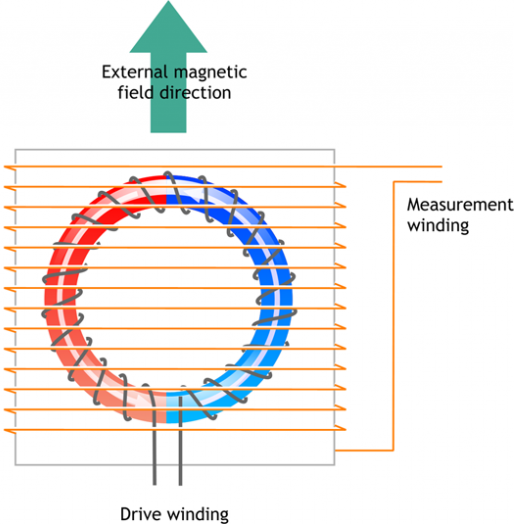
\includegraphics[width=0.6\textwidth]{cassini/FGMdiagram.png}
\caption[Diagram of how a fluxgate magnetometer works.]{Diagram showing basic construction of a fluxgate magnetometer, from \citet{carisma2018}. The drive winding and measurement winding are shown in dark grey and orange, respectively. The magnetic field induced in core due to the current in  the drive winding  is shown by  the pale arrows on top of  the blue and red halves of the  core. The external magnetic field direction is shown by the large green arrow.}
\label{cassini:fig:FGMdiagram}
\end{figure}

The FGM had multiple operational ranges depending on the likely ambient magnetic field strength, which it could switch between automatically, and had a digital resolution of approximately one part in 10,000 depending on the range. The four ranges were $\pm\SI{40}{nT}$ , $\pm\SI{400}{nT}$ , $\pm\SI{10,000}{nT}$, and $\pm\SI{44,000}{nT}$, necessarily for sampling different regions of the magnetosphere and space environment, where the magnetic  field strength  varies over many orders of magnitude. The normal downlink data rate for the FGM was $\SI{32}{vectors/s}$, although in this thesis we only investigate large-scale magnetospheric structures on large timescales, and so only present 1-hour-averaged MAG data.

\subsection{Magnetospheric Imaging Instrument (MIMI)}
The Magnetospheric Imaging Instrument (MIMI) was a system for detecting both neutral and charged particles, described in \citet{krimigis2004} and summarised here. It was composed of three separate instruments, each described below.
\subsubsection{Ion and Neutral Camera (INCA)}
The Ion and Neutral Camera (INCA) could detect either energetic neutral atoms (ENAs) or ion species over the range of energies $\SI{7}{keV/nucleon}<E<\SI{3}{MeV/nucleon}$, and use time-of-flight information to determine the particle's energy and incident direction.

IT works by TBD...

ENAs can be produced via charge exchange between singly-charged energetic ions and Saturn's neutral gas distribution (which originates from Saturn's rings and moons). Through collisions, an energetic ion can `steal' an electron from a neutral particle, such that the ion becomes neutral and is no longer constrained by the planetary magnetic field, and so then travels through space unperturbed. The energetic ions that make up Saturn's equatorial ring current can therefore be traced via detection of ENAs originating from the equatorial plane. Figure~\ref{cassini:fig:INCAringcurrent} shows such an ENA image taken by \textit{Cassini's} MIMI/INCA instrument  on 19 March 2007, clearly showing the variable and substantial ring current structure. 

\begin{figure}
\centering
\noindent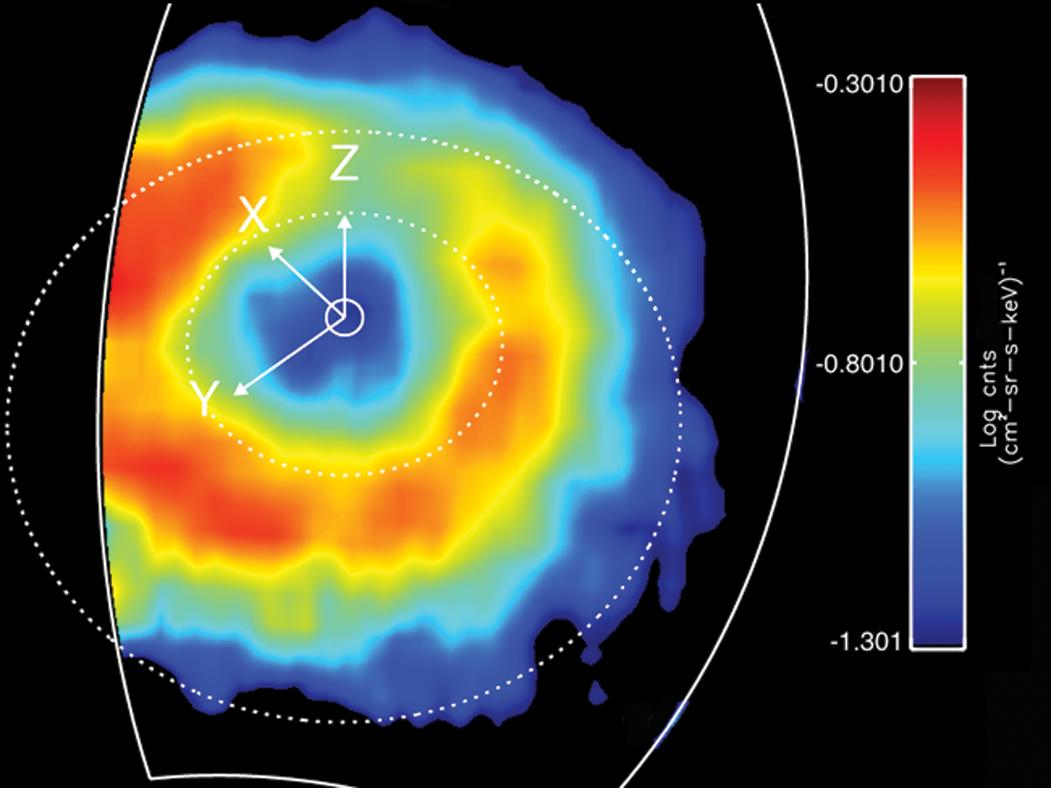
\includegraphics[width=0.8\textwidth]{cassini/INCAringcurrent.jpg}
\caption[ENA image of Saturn's ring current from MIMI/INCA.]{ENA image of Saturn's ring current from the MIMI/INCA instrument as viewed from a latitude of \SI{55}{\degree} above  the northern hemisphere, averaged over a 3 hour period on 19 March 2007. Colour shows ENA intensity as per the colour bar. Saturn is at the  centre, and the white dashed lines show the orbits of the moons Rhea (\SI{8.7}{R_S}) and Titan (\SI{20.2}{R_S}). The Z axis points along Saturn's dipole/spin axis, the Y axis points approximately towards dusk, and the X axis points approximately  towards the Sun. The MIMI/INCA field of view is shown by the solid white line.}
\label{cassini:fig:INCAringcurrent}
\end{figure}

\subsubsection{Charge-Energy-Mass Spectrometer (CHEMS)}
CHEMS measured 
\subsubsection{Low-Energy Magnetospheric Measurement System (LEMMS)}

\subsection{Plasma Spectrometer (CAPS)}
